\documentclass{article}
\usepackage[utf8]{inputenc}
\usepackage[a4paper, margin=1in]{geometry}
\usepackage{fancyhdr}
\usepackage{mathptmx}
\usepackage{multicol}
\usepackage{lipsum}
\usepackage{setspace}
\usepackage{amsfonts}
\usepackage{amsmath}
\usepackage{graphicx}
\usepackage[hidelinks]{hyperref}


\graphicspath{ {./figs/} }

\onehalfspacing

\title{
\noindent\vrule height 2.5pt width \textwidth
\begin{center}
    \bfseries Reinforcement Learning Project
\end{center}
\noindent\vrule height 2.5pt width \textwidth
}
\author{\bfseries Rotem Gazit}
\date{}


\begin{document}

\maketitle


\begin{abstract}
\bfseries
The BipedalWalker environment is considered to be a challenging task in OpenAI's Gym library. The environment consists of a robot with two legs, which is tasked to walk down a 2D track. Here, this environment is resolved using Clipped-Dueling-Double-DQN architecture after only 320 episodes. Moreover, the hardcore version -- which adds obstacles to the path the robot must take, is nearly-resolved ($97.8\%$ of expected score) using the same architecture after 2900 episodes.
\end{abstract}

\begin{multicols}{2}
\section{Introduction}
Reinforcement learning algorithms have significantly evolved in the last decade, and have been successfully applied to a range of challenging problems. DQN based methods allowed to estimate the Q-value, that is the expected future return from a given state and action, even on unmet states -- hence allowing to resolve more complex environments. 

However, the current state-of-the-art methods are much more complex than the popular DQN architecture. The challenge of using DQN-based methods mainly lays in their lack of ability to learn over continuous action spaces, as they are designed to predict the Q-value for all the possible actions $A$ to allow for $\varepsilon$-greedy policies. 

Here, I use DQN-based methods to resolve the BipedalWalker environment. This environment consists of a two-legged robot which is tasked to walk down a given path, with small hills and valleys in the vanilla scenario, and more challenging obstacles in the hardcore version. The robot has some lidar sensors, as well as the velocities of its components. It has control over four motors that move its legs, and is rewarded for moving forward toward the route's end or punished for falling, going backwards or not walking straight.


\subsection{Related Works}
Deep Q-Learning Network (DQN) uses neural networks in order to predict the Q values for every possible action, for a given state, i.e., $f: |S| \to \mathbb{R}^{|A|} \, : \, f(s) = (Q(s,a_1), \dots, Q(s,a_{|A|}))$ where $S, A$ denote the possible states and actions of the environment, respectively. 
Under the hood, DQN consists of multiple neural network layers, and we update their weights according to the accuracy of the predicted Q-values, when compared to actual rewards, in a manner similar to Self-Supervised learning methods \cite{DQN}. 

This process tends to be quite noisy and hard to "tame", and numerous improvements were suggested in recent years. \textbf{Double Deep Q-Learning Network} (DDQN) utilizes two DQN networks -- the first one is used to pick the next action, and the other is used to predict the Q-value of the state and the chosen action \cite{DDQN}. 
$$Q^*(s_t, a_t) = r_t + \gamma Q_{\theta'}(s_{t+1}, \arg \max_{a'}Q_{\theta}(s_{t+1}, a'))$$
Where $s_t, a_t, r_t$ are the state, action and reward observed at time $t$, $\theta, \theta'$ are the weights of the DQN and target network, and $\gamma$ is the discount factor.
Every few episodes, we copy the weights of the first network into the other. DDQN reduces the amount of noise created during training and assists in reaching better results faster, hence it is widely used.

\textbf{Clipped Double Q Learning} is a variant of DDQN, which was originally introduced for Action-Critic methods \cite{ClippedDQN}. Here, two networks are trained simultaneously, using the minimal Q-value they return \cite{ren2021on}. 
$$Q^*(s_t, a_t) = r_t + \gamma \min_{\{i = 1, 2\}} (Q_{\theta'_i}(s_{t+1}, \arg \max_{a'}Q_{\theta_1}(s_{t+1}, a')))$$
Where $s_t, a_t, r_t$ are the state, action and reward observed at time $t$, $\theta_{\{1,2\}},  \theta'_{\{1,2\}},$ are the weights of the DQN and target network, and $\gamma$ is the discount factor.

Another known improvement is \textbf{Dueling DQN}, which instead of predicting $Q$ directly, predicts $Q(s,a)=V(s)+A(s,a)$, i.e, the \textit{value} of state $s$ (regardless of the chosen action), and the \textit{advantage} of picking action $a$ \cite{DuelingDQN}. In practice, two parallel dense layers are being added to the network -- one to evaluate $V$ and the other to evaluate $A$, and the combination $Q(s,a)=V(s)+A(s,a) - \frac1{|A|}\sum_{a'\in A}A(s,a')$ is the final result we use for training.

Offline learning methods use Replay Buffer in order to sample historical observations for training \cite{DQN}. As the size of replay buffer increases, the need for making sure the best observations are picked for training emerges. A common practice is to use a Prioritized Experience Replay (PER) \cite{PER}, which uses the error in predicting the Q-value for each state as the weights in picking a sample of them. Another newer approach achieves similar results to PER, but remove the need for the more complex sampling process, by always slightly biasing the samples taken to more recent observations \cite{ExpReplay}.

Stacking multiple solutions together has showed significant improvement in the performance \cite{Rainbow}. Previous works have shown that together these approaches can resolve many complex environments successfully.

DQN has some adaptations into continuous action spaces. Normalized Advantage Functions (NEF) adapts the Dueling-DQN model into continuous spaces by changing the advantage component \cite{NEF}.
It defines the advantage as $A(s,a) = \frac12 (a-\mu(s))^T P(s) (a - \mu(s))$, where $P=L(s)L(s)^T$, $L(s)$ is a state-dependent lower-triangular matrix that we predict and $\mu(s)$ is the next action that we take. $\mu(s) \in A$ is designed to be the action that maximizes the Q-value for the state, $\mu(s) = {\arg \max}_{a\in A} Q(s,a)$. NEF maintains a single-network architecture, unlike Actor-Critic models, which makes it simpler to implement as there are less hyperparameters to optimize.

\section{Solution}

\subsection{General Approach}
In order to solve the described environment, I combined several methods into a model-free, off-line, Clipped-Dueling-Double-DQN, which is able to resolve the Bipedal Walker environment in $\sim 300$ episodes, and nearly-resolve the hardcore version in $\sim 3000$ episodes (see section \ref{section:results}).


\subsection{Design}
\subsubsection{Clipped Dueling DDQN}
The Dueling DQN and Clipped Double DQN were combined in order to create the \textbf{Clipped Dueling DDQN} architecture used to solve both the normal Bipedal Walker and the hardcore environments.

In practice, two networks $Q_{\theta_1}, Q_{\theta_2}$ are trained, where their final layers are a combination of two streams of $V$ and $A$: $Q(s,a)=V(s)+A(s,a) - \frac1{|A|}\sum_{a'\in A}A(s,a')$. Moreover, two target networks $Q_{\theta'_1}, Q_{\theta'_2}$ are kept as well, and every $\tau$ steps the weights of $Q_{\theta_i}$ are copied to $Q_{\theta'_i}$. $Q_{\theta_i}$ are trained over the clipped Q-value: 
$$Q^*(s_t, a_t) = r_t + \gamma \min_{\{i = 1, 2\}} (Q_{\theta'_i}(s_{t+1}, \arg \max_{a'}Q_{\theta_1}(s_{t+1}, a')))$$
The network itself consists of 3 layers with $[512, 512, 256]$ neurons, using ReLU as the activation method (Figure \ref{fig:network}).

This method combines several approaches for minimizing the overestimation of Q-values, allowing for relatively swift and stable training.

\begin{figure*}
\begin{center}


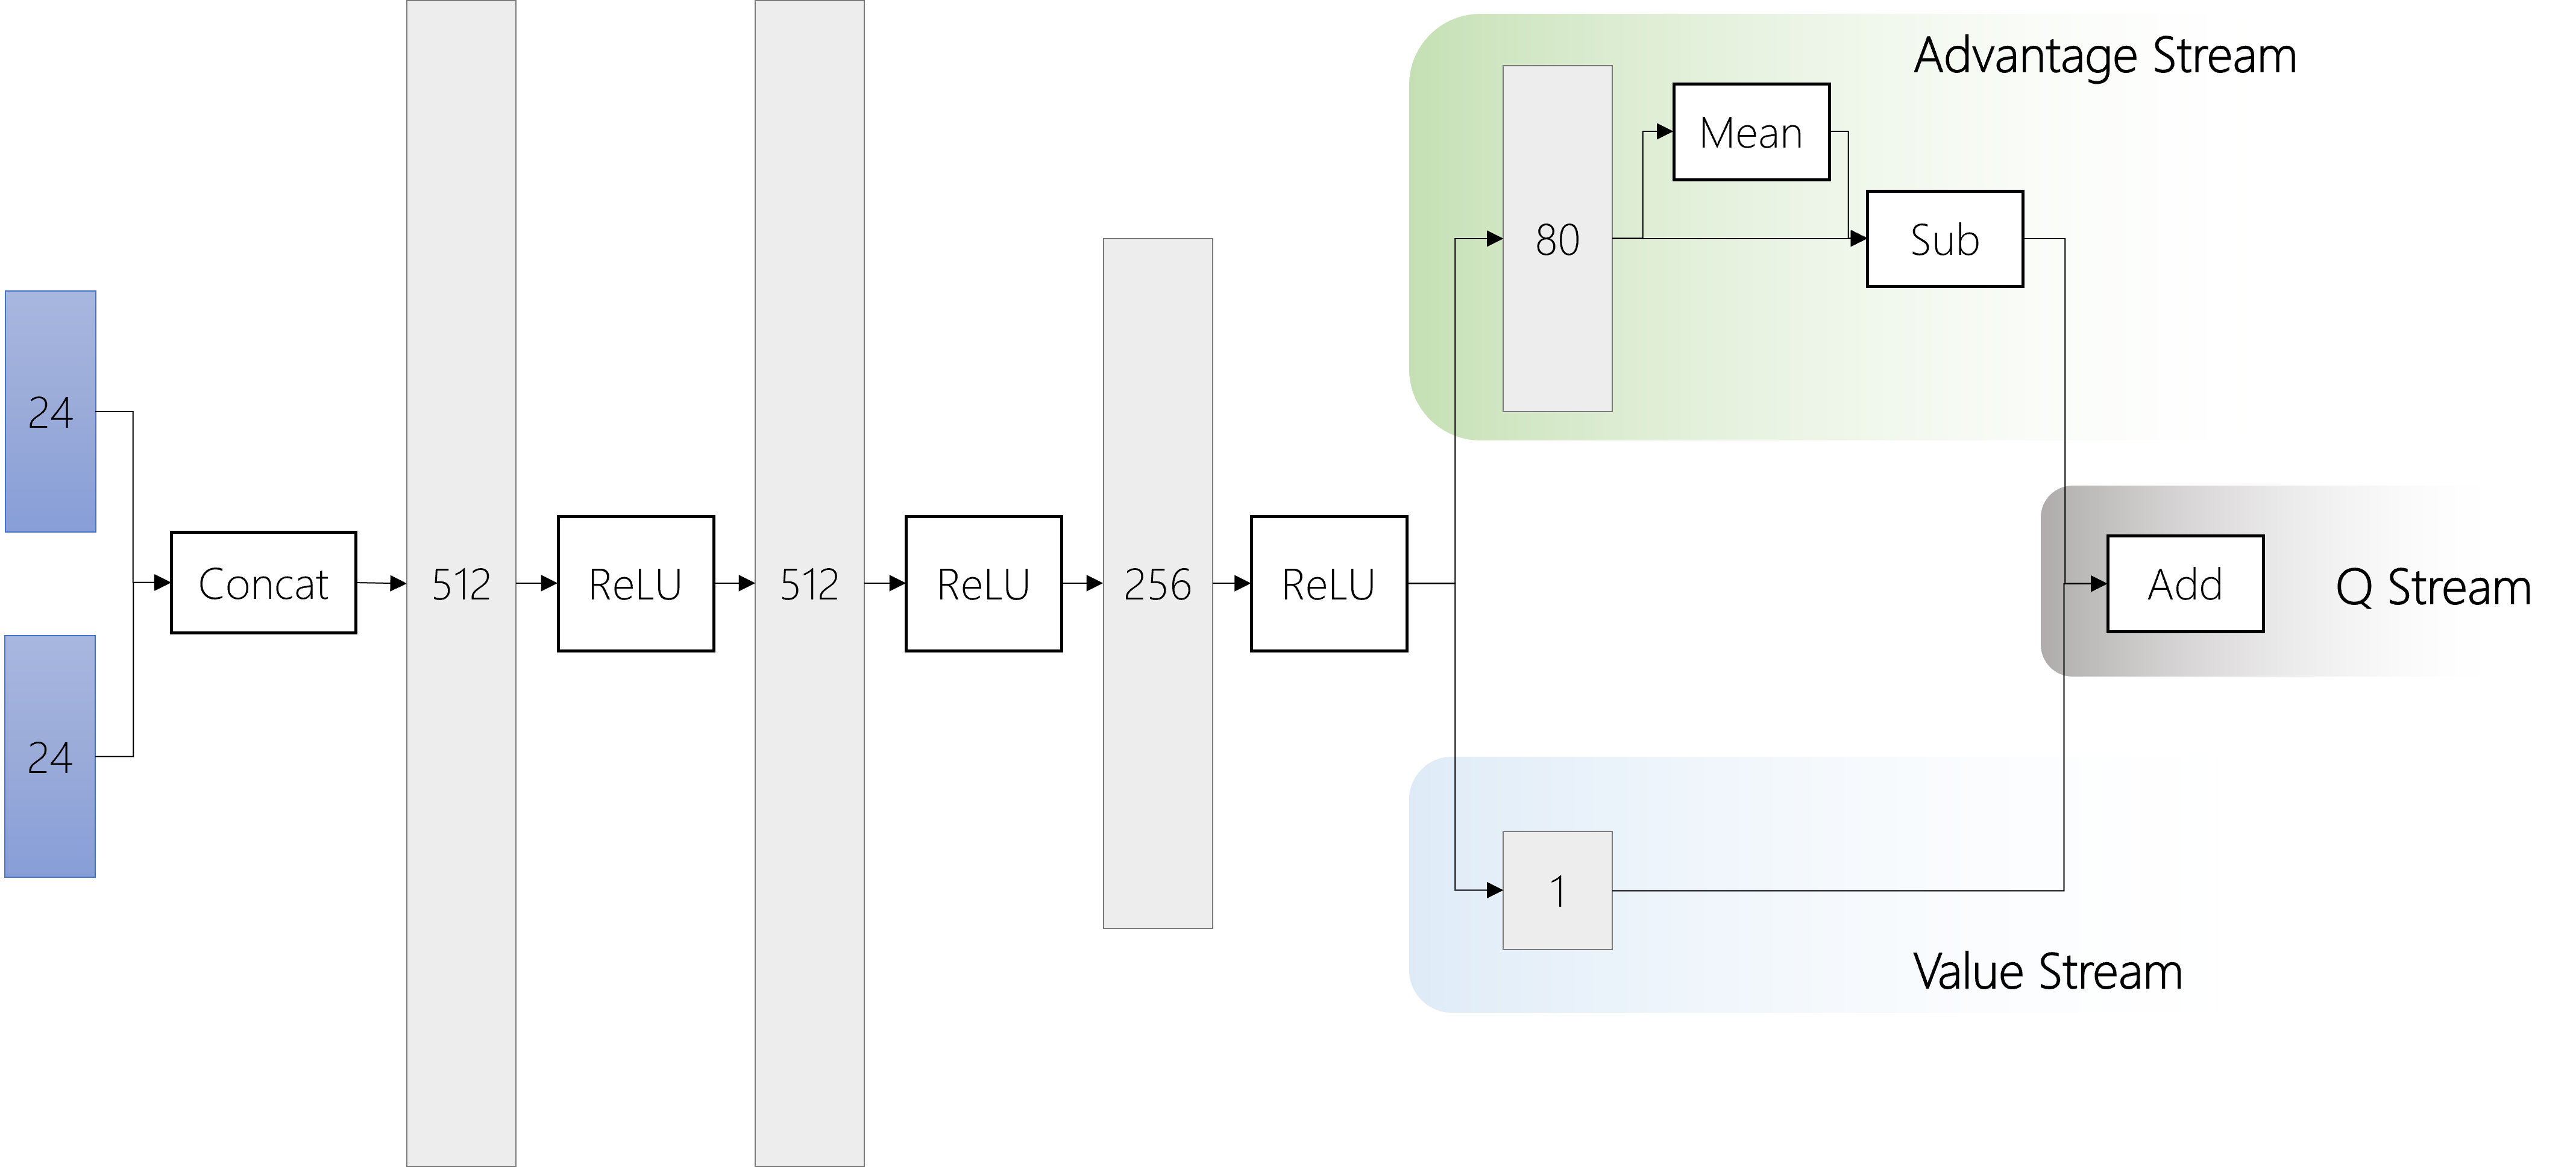
\includegraphics[width=0.8\textwidth]{network}
\caption{\label{fig:network}
\textbf{Network Architecture}
}
\end{center}
\end{figure*}

\subsubsection{Action Space}
The action space of the Bipedal Walker contains 4 continues axes: $A=[-1,1]^4$. But since DQN-based learning methods can only cope with discrete action spaces, some kind of discretization must take place beforehand. It is important to note that too many possible actions would require longer training and exploration, hence One needs to decide whether it is more effective to have higher-resolution control over each axis, or to have multiple axes activated at the same time. Eventually I found that preferring axes combination produces better result than having more sensitive control over each individual axes. Moreover, I found that removing the "null action" $(0,0,0,0)$ also improves the results of the model (as the agent is not able to "rest" at any point in time, hence must keep moving).
The final action space is $\bar{A}=\{-1,0,1\}^4 \setminus \{0\}^4 \subset A$, which has $|\bar{A}|=80$ possible actions.

\subsubsection{State Preprocessing}
The observation-space of the Bipedal Walker environment is limited to several sensors the robot contains, mainly sensors that capture limited information about the environment and velocities of several components. In order to compensate about the lack of acceleration metrics, I combined $k$ consecutive frames into a single state. After picking an action $a$, it is applied $k$ times in order to create the next state. After several trials, I decided using $k=2$, which makes each state a vector of $48$ elements. 
In order to speed up training, I found it unnecessary to train after each state - especially when using large batch size and long episodes. Instead, training is only done every other state.

Since some of the features aren't explicitly bounded, I found it necessary to normalize them all to consistent scales. I used the standard normalization, $\bar{x}_i = \frac{x_i - \hat{\mu}_i}{\hat{\sigma}_i}$, where $x_i$ is the $i$-th feature, and $\hat{\mu}_i, \hat{\sigma}_i$ are the observed mean and standard deviation, which are being updated during the initial random exploration before training. This normalization helps in preventing the gradients from exploding as the agent approached undiscovered territory.

\subsubsection{Reward Preprocessing}
In the BipedalWalker environment, the reward for each action varies - most of the time it is quite small ($|r| \leq 1$), but when if the robot touches the ground it receives a penalty of $-100$ points. The large variety in scales introduces noise into the learning process. As previous articles have reported, normalizing the rewards can help to utilize higher learning rates and reduce fluctuations in the learning process. Here, The reward was clipped into the range $[-10, 1]$ and normalized using their empirical standard deviation, which is updated in the initial stages of training (similarly to the way state features are being normalized), i.e., $\bar{r}_i = \frac{\text{clip}(r_i, -10, 1)}{\hat{\sigma}}$. Note that the mean reward isn't in use, as the sign of the reward $r$ is important to maintain.

\subsubsection{Experience Replay Buffer}
Experience Replay Buffer is an important component for off-line learning algorithms. It stores the last previous $N$ tuples of states, action taken, rewards, and following states, denoted $(s_t, a_t, r_t, s_{t+1})$. Here, I created a buffer of the last $N=1{\small ,}000{\small ,}000$ tuples, in order to learn over long-forgotten experiences. 

Large replay buffers, although help in creating a long-term memory, suffer from different problems -- the current policy is hardly ever challenged directly since the odds of picking recent experiences is low. A common improvement is to use Prioritized Experience Replay buffers (PER) \cite{PER}, which are designed to pick experiences with higher prediction errors. Here, I use a newer approach that achieved similar results \cite{ExpReplay} -- Instead of picking a random batch of $B$ tuples from the replay buffer, $B-1$ random tuples are sampled and combined with the last observed tuple. This creates $B$ tuples for the network to train over, which are slightly biased toward the most recent state it reached.

\subsubsection{Loss Function and Optimizer}
Non-stationary learning tasks, such as reinforcement learning, might not benefit from momentum-based optimizers, since the target is not fixed throughout the training, hence making the momentum misleading. I find that using RMSProp, which does not contain any momentum component, helps in stabilizing the results faster. I also used gradient clipping to avoid drastic changes in the weights of the network. The loss function used is the standard Mean Squared Error (MSE).

\subsubsection{Biased $\epsilon$-Greedy}
Discrete reinforcement learning algorithms have hard time in utilizing large action spaces. $\epsilon$-greedy makes exploration rarer over time, which makes it harder to detect better strategies. Here, actions are sampled unevenly, biased toward less explored actions. Let $p_i$ be the relative frequency of $a_i \in A$ in replay buffer $\mathfrak{D}$, $p_i = \frac{|\{d \in \mathfrak{D}\ :\ a_i \in d \}|}{|\mathfrak{D}|}$.
Let $\hat{p}_i = \frac{1 - p_i}{\sum_i 1 - p_i}$, whenever a random action needs to be picked according to the $\epsilon$-greedy policy, I sample actions according to $\mathbb{P}(a_t = a_i) = \hat{p}_i$.

\subsubsection{BipdealWalker as Non-Episodial Task}
The BipdealWalker environment has a finite track the robot must run through. However, there are no apparent features that define the end of that track, according to the robot's sensors. Theoretically, the track could have been endless, and the robot could run forever. 

If the end of the track is regarded as a terminal state, the Bellman Equation used in DQN-based methods would actually punish the robot for reaching there. 
Let $s_t, r_t, a_t$ an observed state, reward and action, where $s_{t+1}$ is observed when the robot reached the end of the track. Since there are no apparent characteristics in the observed $s_t, s_{t+1}$ that allows to predict beforehand that the robot reaches the end, we might observe $s'_k, s'_{k+1}, s_t \approx s'_k, s_{t+1} \approx s'_{k+1}$ in mid-track. In this case, DQN would be trained over $Q^*(s_t, a_t) = r_t$, as well as $Q^*(s'_k, a'_k) = r'_k + \gamma V(s'_{k+1}) \gg Q^*(s_t, a_t)$. This unnecessary noise during training can be avoided if reaching the end of the track is not regarded as a terminal state.

Therefore, the only terminal state in training is when the robot touches the ground. Otherwise, the network is trained as if the route is endless, but episodes still end whenever the robot reaches the final line.

\subsubsection{Hyperparameters Optimization}
Hyperparameters were optimized using Optuna, which was tasked to find the right learning rate for achieving the highest average reward in the last $10$ episodes. The batch size was fixed to $128$, and the discount factor $\gamma$ was set to $0.99$.
The balance between exploration and exploitation was achieved by selecting actions using the $\varepsilon$-greedy strategy, where the initial value of $\varepsilon$ was $1$, and it decayed after each episode $t$ by $\varepsilon_{t+1} = \max\{0.99\varepsilon_t, 0.01\}$.

\subsubsection{Solving BipdealWalker-Hardcore}
The hardcore variant of the BipdealWalker environment adds obstacles to the track, which demands to robot to change its reaction according to its limited sensors. Eventually, the same model architecture was used for both the vanilla and the hardcore versions, but many of the architecture features derived from trying to resolve the hardcore environment.

Several alternative approaches were examined when trying to resolve the hardcore variant. 
First, I tried to decrease the size of the action space by reframing the problem as 4 different "agents" -- one for each axis the robot can control. I trained 4 different Q-value streams, each for every axis, which allowed for each stream to have only 3 discrete actions: $\{-1, 0, 1\}$. This method could not learn any complex strategies, as it greedily picks the best action from each axis, and misses wiser combinations of the four, saturating in an average score of $\sim 198$.

Next, I tried to learn over the original continuous action space. I examined Normalized Advantage Functions (NEF) that adapts the Dueling-DQN model into continuous spaces, but unlike methods such as Actor-Critic, it maintains a simpler single-network architecture \cite{NEF}. 
This method has reached the track's end successfully and consistently, but failed to learn how to balance the robot's "head" and therefore suffered from large penalties from the environment, saturating in an average score of $\sim 270$.

Finally, after adding the introducing the improved action exploration, terminal state definition and Clipped-DQN architecture, I was able to nearly-resolve the hardcore version using the discrete action space used for the vanilla variant.

\subsection{Experimental Results}
\label{section:results}
 The model was trained using batch size of 128 observations. Every 10 episodes, the model was evaluated by playing 20 consecutive games, i.e., only with greedy policy. Training was stopped after the evaluation achieved an average score of 300.
 
 The vanilla environment was resolved after 320 episodes, and the hardcore environment was nearly-resolved after 2900 episodes -- reaching $293.476$ average score (Figure \ref{fig:scores}).
 
 \begin{figure*}
 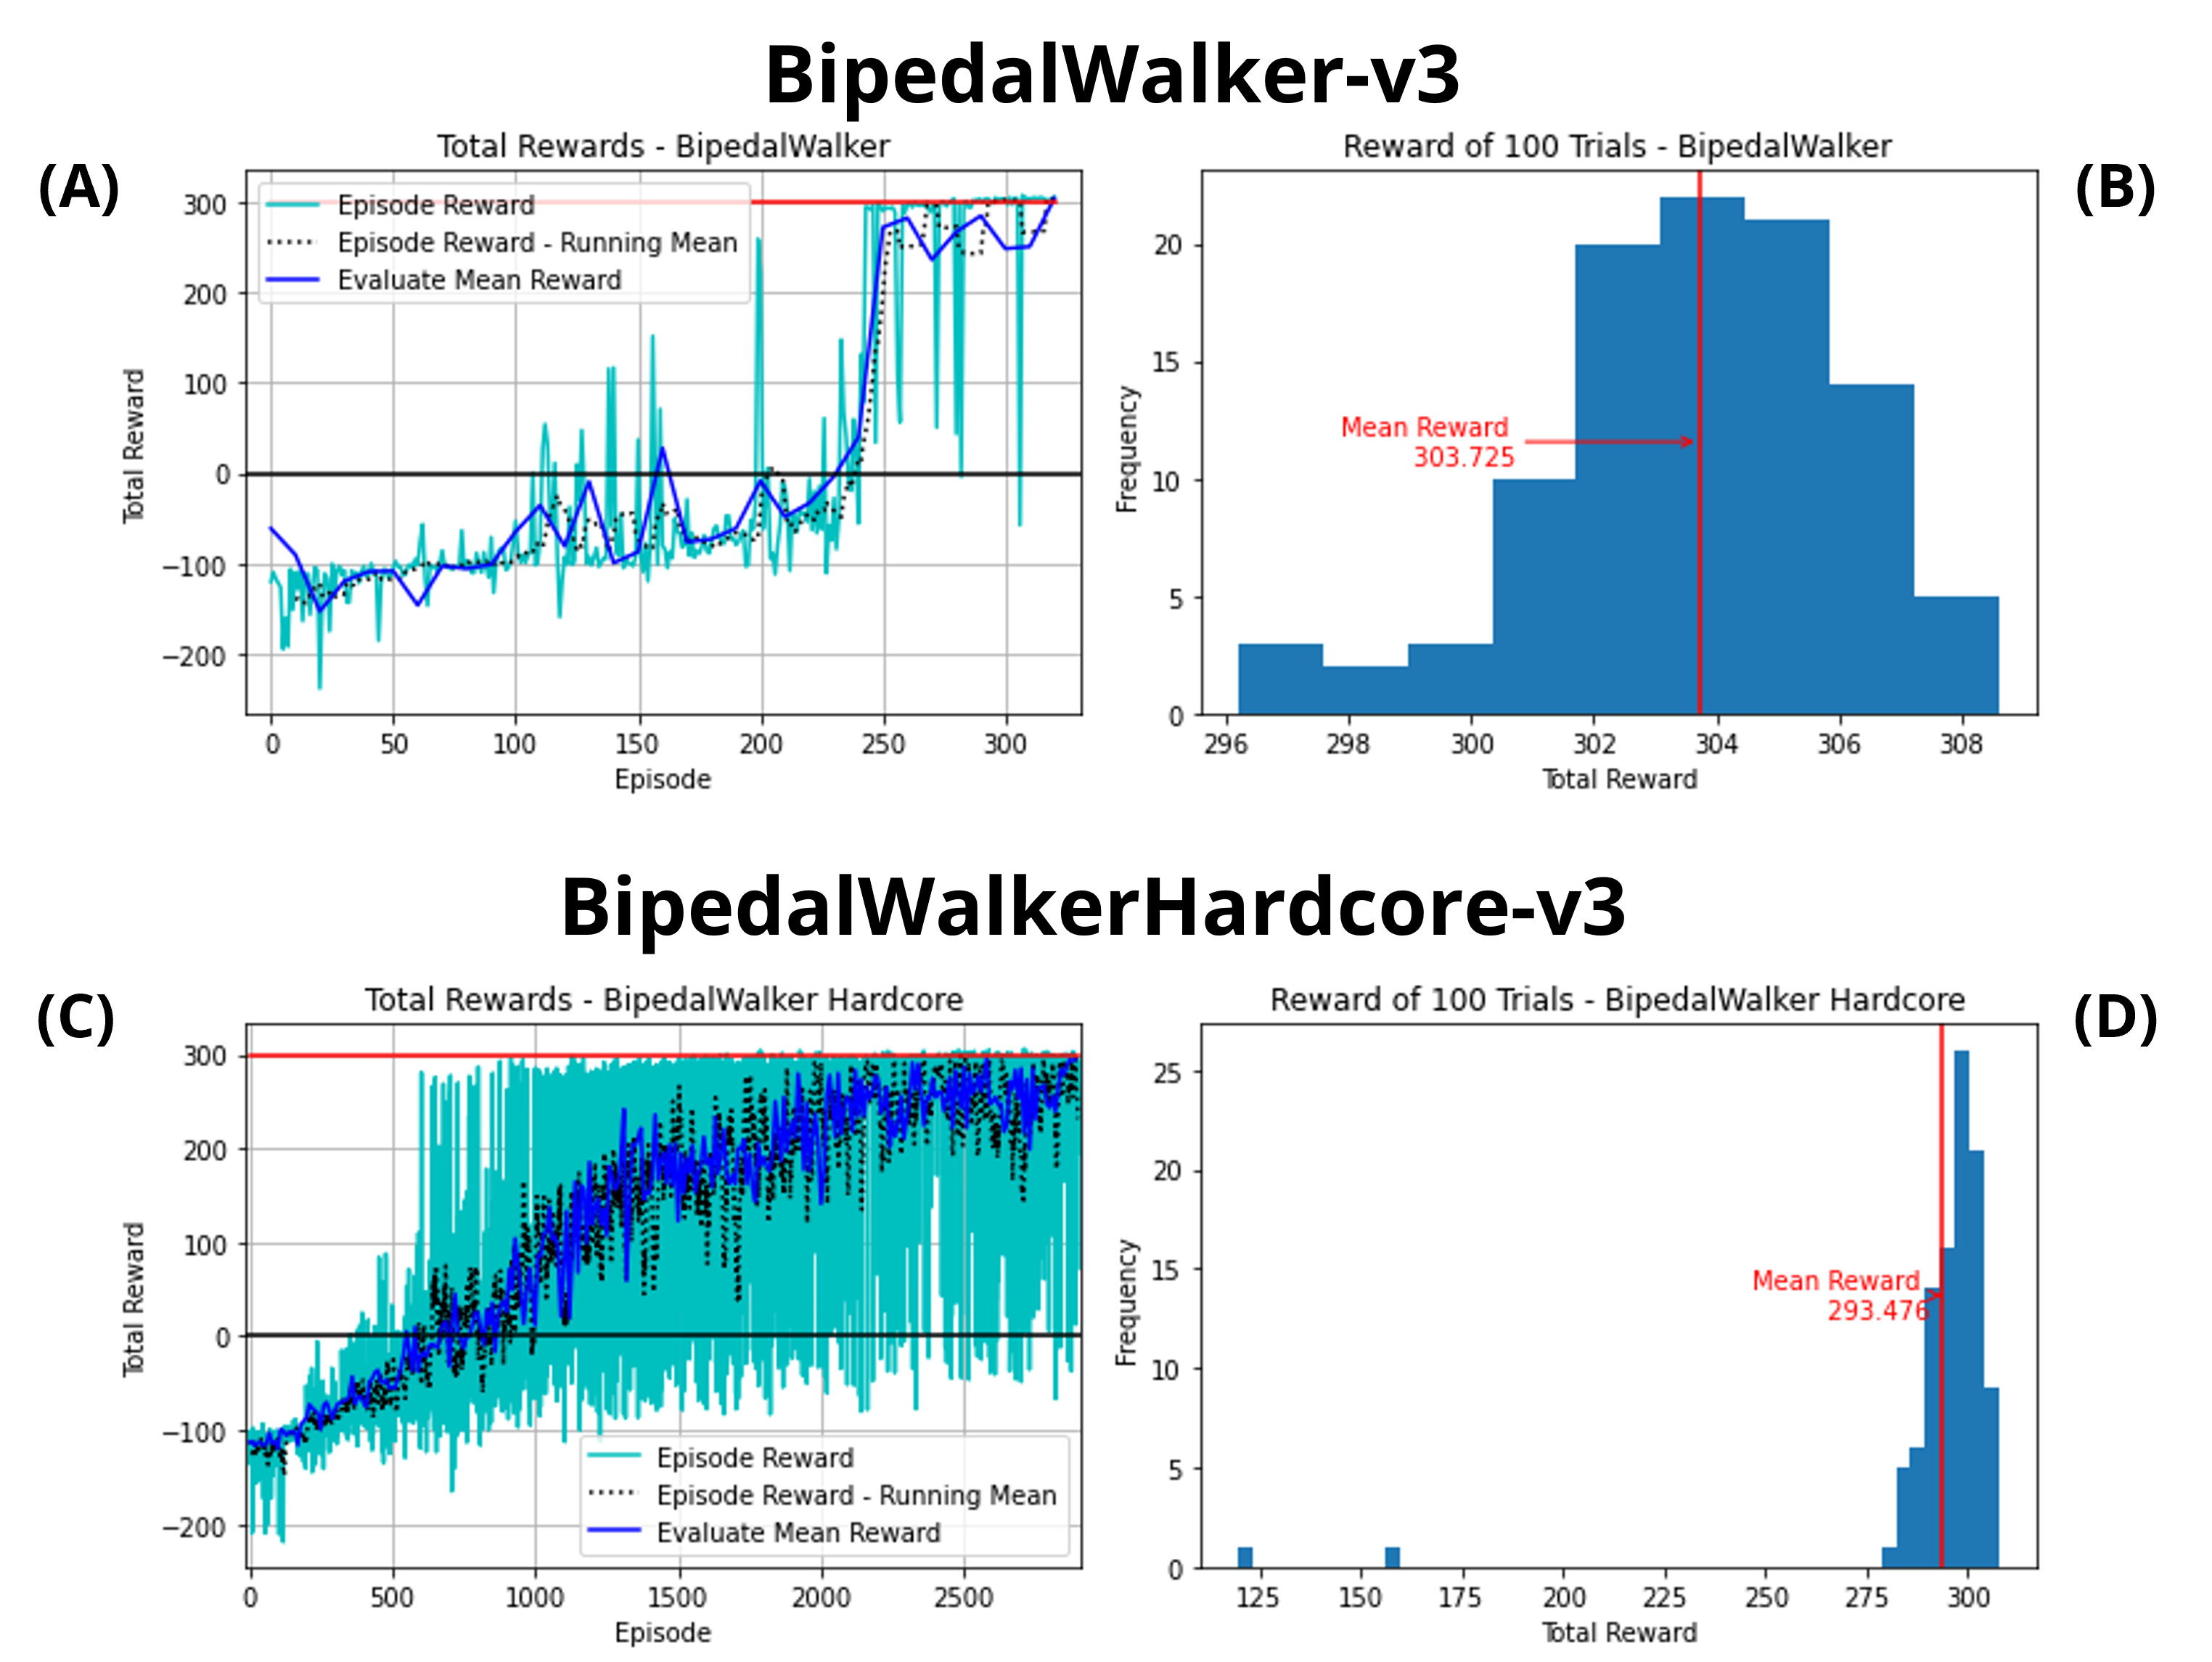
\includegraphics[width=\textwidth]{scores}
 \caption{
 \label{fig:scores}
 \textbf{Results of BipdealWalker and BipedalWalkerHardcore.} \\
 \textbf{(A)} Total rewards of vanilla environment during training and evaluation. The total reward of each episode (cyan) first reaches the target value of 300 at episode 274 and stabilizes at episode $\sim 280$. The evaluation over 100 consecutive trials (blue) crosses the 300 threshold at episode $320$. \\
 \textbf{(B)} The histogram of total rewards of 100 evaluation games. The mean total reward is above 300, which means the model has successfully resolved this environment. \\
 \textbf{(C)} Similarly to (A), the total rewards of the hardcore environment during training and evaluation. The total reward of each episode (cyan) first reaches the target value of 300 at episode 1648 and stabilizes at episode $\sim 2500$. The evaluation over 100 consecutive trials (blue) was nearest to the 300 theshold ($293.476$) at episode 2900. \\
 \textbf{(D)} Similarly to (B), the histogram of total rewards of 100 evaluation games for the hardcore version. The mean total reward is above $293.476$, which means the model has nearly-resolved this environment.
 }
 \end{figure*}
 
\section{Discussion}
The BipdealWalker environment, due to the limited sensors of the robot, is a challenging reinforcement learning task to overcome. Here, using only discrete action spaces, I was able to solve both the vanilla, and nearly-resolve the hardcore variants of the environment. Using a collection of different approaches, the final model was powerful enough to learn and generalize from experiences.

The vanilla variant of the BipdealWalker was easy enough to solve in a small number of episodes, even with simpler architectures. Although the original action space is continuous, discretizing in into $\{-1, 0, 1\}^4$ was enough for reaching excellent results. This led me to believe that even the hardcore version could be resolved without changing the architecture into continuous models. After stacking multiple improvements together, that allowed for better exploration and prevent the model from over-estimating states, I was able to nearly-resolve even the hardcore version using the simpler discrete action space -- and I believe a full resolution of the environment would emerge if more episodes were allowed. As the current state-of-the-art models are Actor-Critic approaches, achieving these results using simpler DQN models was refreshing and some-what surprising.

\section{Code}
The full code can be found here: \href{https://colab.research.google.com/drive/1_gxpvbnFv3lCQh4Ce_f1osPcGhwog27W?usp=sharing}{LINK}

\bibliographystyle{apalike}
\bibliography{ref}

\end{multicols}



\end{document}
